\documentclass[conference]{IEEEtran}
\IEEEoverridecommandlockouts
% The preceding line is only needed to identify funding in the first footnote. If that is unneeded, please comment it out.
\usepackage{cite}
\usepackage{amsmath,amssymb,amsfonts}
\usepackage{algorithmic}
\usepackage{graphicx}
\usepackage{tikz}
\usepackage{pgfplots}
\pgfplotsset{compat=1.18}
\usepackage{textcomp}
\usepackage{subfig}
\usepackage{xcolor}
\usepackage{multirow}
\def\BibTeX{{\rm B\kern-.05em{\sc i\kern-.025em b}\kern-.08em
    T\kern-.1667em\lower.7ex\hbox{E}\kern-.125emX}}
\begin{document}

\title{Mémoires caches - Evaluation des performances de différentes
configurations de mémoires caches\\
}

\author{\IEEEauthorblockN{1\textsuperscript{st}  Luiz Gariglio Dos Santos }
\IEEEauthorblockA{\textit{Ingénieur Degree Programme in STIC} \\
\textit{ENSTA Paris}\\
Paris, France \\
email@ensta-paris.fr}
\and
\IEEEauthorblockN{2\textsuperscript{nd} Helena Guachalla De Andrade}
\IEEEauthorblockA{\textit{Ingénieur Degree Programme in STIC} \\
\textit{ENSTA Paris}\\
Paris, France \\
email@ensta-paris.fr}
\and
\IEEEauthorblockN{3\textsuperscript{rd} Santiago Florido Gomez}
\IEEEauthorblockA{\textit{Ingénieur Degree Programme in STIC} \\
\textit{ENSTA Paris}\\
Paris, France \\
santiago.florido@ensta-paris.fr}
\and
\IEEEauthorblockN{4\textsuperscript{th} Franck Ulrich Kenfack Noumedem}
\IEEEauthorblockA{\textit{Ingénieur Degree Programme in STIC} \\
\textit{ENSTA Paris}\\
Paris, France \\
email@ensta-paris.fr}
}

\maketitle

\begin{abstract}
Ce rapport analyse l’influence de la hi\'erarchie m\'emoire et des contraintes \'energ\'etiques sur les performances des processeurs. Dans un premier temps, nous \'evaluons l’impact des caches L1/L2 sur des calculs matriciels, en mettant en \'evidence le r\^ole cl\'e de la localit\'e et de l’organisation des donn\'ees. Dans un second temps, nous menons une exploration de l’espace de conception d’une architecture \emph{big.LITTLE} (Cortex-A7/A15) afin d’optimiser les configurations pour Dijkstra et Blowfish. Les performances sont mesur\'ees avec Gem5 (IPC, taux de \emph{miss}) et les co\^uts physiques des caches sont estim\'es avec CACTI, compil\'e en version~7.0 pour fiabiliser les r\'esultats en 32~nm.

\end{abstract}

\begin{IEEEkeywords}
Memory Wall, hi\'erarchie m\'emoire, caches L1/L2, localit\'e m\'emoire, Gem5, CACTI, Design Space Exploration (DSE), big.LITTLE, Cortex-A7, Cortex-A15, IPC, taux de \emph{miss}, Dijkstra, Blowfish
\end{IEEEkeywords}




\section{Introduction}

Dans le contexte actuel des syst\`emes embarqu\'es et du calcul haute performance, la conception de processeurs est confront\'ee \`a deux contraintes majeures : le \emph{mur m\'emoire} (\emph{Memory Wall}), qui limite les gains de performance lorsque la hi\'erarchie m\'emoire ne suit pas le rythme du calcul, et l’efficacit\'e \'energ\'etique, devenue d\'eterminante pour les plateformes modernes. Ce rapport de travaux pratiques s’articule autour de deux \'etudes compl\'ementaires visant \`a caract\'eriser et quantifier ces probl\'ematiques \`a travers des exp\'erimentations reproductibles.

La premi\`ere partie (Exercice~3) analyse l’impact de la hi\'erarchie m\'emoire (caches L1/L2) sur des algorithmes de calcul matriciel. L’objectif est de montrer que les performances ne d\'ependent pas uniquement de l’algorithme, mais aussi de la mani\`ere dont les donn\'ees sont organis\'ees et acc\'ed\'ees en m\'emoire, notamment via la localit\'e spatiale et temporelle.

La seconde partie (Exercice~4) porte sur une exploration de l’espace de conception (\emph{Design Space Exploration}, DSE) appliqu\'ee \`a une architecture h\'et\'erog\`ene \emph{big.LITTLE}. Nous dimensionnons un cluster \emph{LITTLE} (Cortex-A7) et un cluster \emph{big} (Cortex-A15) pour des charges applicatives distinctes (Dijkstra et Blowfish), en mettant en \'evidence les compromis entre performance, co\^ut en surface et consommation.

Pour mener ces analyses, nous nous appuyons sur deux outils principaux : Gem5, utilis\'e en mode \emph{Syscall Emulation} pour simuler l’ex\'ecution et extraire des indicateurs tels que l’IPC et les taux de \emph{miss}, et CACTI, utilis\'e pour estimer la surface et l’\'energie des caches. Enfin, afin de garantir la fiabilit\'e des r\'esultats de l’Exercice~4, nous avons automatis\'e les campagnes de simulation et pris l’initiative de compiler CACTI~7.0, ce qui a permis de corriger des erreurs critiques observ\'ees avec la version standard lors des estimations en technologies fines (notamment 32~nm).


\section{Evaluation des performances de différentes
configurations de mémoires caches pour 4
algorithmes de multiplication de matrices}

    \subsection{Paramètres de configuration des caches utilisés dans gem5}
    
        \begin{table}[h]
            \centering
            \footnotesize
            \setlength{\tabcolsep}{3pt}
            \resizebox{\linewidth}{!}{%
                \begin{tabular}{|c|c|c|c|c|}
                    \hline
                    \textbf{Configuration} & \textbf{Instruction cache}                                   & \textbf{Data cache}                                           & \textbf{L2 cache}                                              & \textbf{Block size} \\ \hline
                    C1                     & \begin{tabular}[c]{@{}c@{}}4KB \\ direct-mapped\end{tabular} & \begin{tabular}[c]{@{}c@{}}4KB \\ direct-mapped\end{tabular}  & \begin{tabular}[c]{@{}c@{}}32KB \\ direct-mapped\end{tabular}  & 32 bytes                          \\ \hline
                    C2                     & \begin{tabular}[c]{@{}c@{}}4KB \\ direct-mapped\end{tabular} & \begin{tabular}[c]{@{}c@{}}4KB \\ 2-way set-asso\end{tabular} & \begin{tabular}[c]{@{}c@{}}32KB \\ 4-way set-asso\end{tabular} & 32 bytes                         \\ \hline
                \end{tabular}
            }
            \caption{}
        \end{table}
        
        Les paramètres de configuration des caches dans le simulateur gem5 suivent le format suivant :
        {\footnotesize\texttt{tag:\allowbreak n\_lignes:\allowbreak taille\_bloc:\allowbreak associativite:\allowbreak politique}}.
        
        Pour chaque cache, le nombre de lignes est obtenu en divisant la taille totale du cache par la taille d’un bloc. 
        L’associativité correspond au nombre de voies, fixé à 1 pour un cache direct-mapped, 2 pour un cache 2-way set-associative, etc. Enfin, la politique de remplacement utilisée ici est LRU, notée \texttt{l}.
        
        Ainsi, pour la configuration C1, par exemple, le cache d'instructions possède \(\frac{4096}{32} = 128\) lignes, d'où \texttt{il1:128:32:1:l}. En utilisant la même logique pour les autres caches et configurations, le tableau suivant est rempli.
        
        \begin{table}[h]
            \centering
            \footnotesize
            \setlength{\tabcolsep}{3pt}
            \begin{tabular}{|c|c|c|c|}
                \hline
                \textbf{Configuration} & \textbf{IL1}   & \textbf{DL1}   & \textbf{UL2}    \\ \hline
                C1                     & il1:128:32:1:l & dl1:128:32:1:l & ul2:1024:32:1:l \\ \hline
                C2                     & il1:128:32:1:l & dl1:64:32:2:l  & ul2:256:32:4:l  \\ \hline
            \end{tabular}
        \end{table}
    
    \subsection{Taux de défauts dans les différentes caches}
    
        \begin{itemize}
            \item Le taux de défauts dans le cache d’instructions il1 : \texttt{icache.overallMissRate}
            \item Le taux de défauts dans le cache de données dl1 : \texttt{dcache.overallMissRate}
            \item Le taux de défauts dans le cache unifié (L2) ul2 : \texttt{l2cache.overallMissRate}
        \end{itemize}
        
        \begin{table}[h]
            \centering
            \footnotesize
            \setlength{\tabcolsep}{3pt}
            \begin{tabular}{|c|c|c|}
                \hline
                \multirow{2}{*}{\textbf{Programmes}} & \multicolumn{2}{c|}{\textbf{Configuration de caches}} \\ 
                \cline{2-3} 
                                                        & C1       & C2             \\ \hline
                P1 normale                           & $ 0,00\%$         &  $ 0,00\%$    \\ \hline
                P2 (pointeur)                        & $ 0,00\%$         &  $ 0,00\%$   \\ \hline
                P3 (tempo)                           & $ 0,00\%$         &  $ 0,00\%$   \\ \hline
                P4 (unrol)                           & $ 0,00\%$         &  $ 0,00\%$   \\ \hline
            \end{tabular}
            \caption{icache.overallMissRate}
            \label{tab:icache}
        \end{table}
        
        \begin{table}[h]
            \centering
            \footnotesize
            \setlength{\tabcolsep}{3pt}
            \begin{tabular}{|c|c|c|}
                \hline
                \multirow{2}{*}{\textbf{Programmes}} & \multicolumn{2}{c|}{\textbf{Configuration de caches}} \\ 
                \cline{2-3} 
                                                        & C1       & C2             \\ \hline
                P1 normale                           & $ 30,08\%$         &  $ 31,01\%$    \\ \hline
                P2 (pointeur)                        & $ 30,22\%$         &  $ 31,12\%$   \\ \hline
                P3 (tempo)                           & $ 30,23\%$         &  $ 31,12\%$   \\ \hline
                P4 (unrol)                           & $ 30,06\%$         &  $ 31,10\%$   \\ \hline
            \end{tabular}
            \caption{dcache.overallMissRate}
        \end{table}
        
        \begin{table}[h]
            \centering
            \footnotesize
            \setlength{\tabcolsep}{3pt}
            \begin{tabular}{|c|c|c|}
                \hline
                \multirow{2}{*}{\textbf{Programmes}} & \multicolumn{2}{c|}{\textbf{Configuration de caches}} \\ 
                \cline{2-3} 
                                                        & C1       & C2             \\ \hline
                P1 normale                           & $ 43,85\%$         &  $ 42,20\%$    \\ \hline
                P2 (pointeur)                        & $ 43,63\%$         &  $ 42,21\%$   \\ \hline
                P3 (tempo)                           & $ 43,62\%$         &  $ 42,20\%$   \\ \hline
                P4 (unrol)                           & $ 43,65\%$         &  $ 42,02\%$   \\ \hline
            \end{tabular}
            \caption{l2cache.overallMissRate}
        \end{table}

        Nous pouvons vérifier que les quatre algorithmes présentent une bonne localité de référence pour le code. 
        En effet, le taux de défaut du cache d’instructions est nul $(\approx 0,00\%)$ pour tous les programmes et 
        pour les deux configurations de caches (Table \ref{tab:icache}). Cela signifie que le flux d’instructions 
        tient entièrement dans le cache d’instructions et que les boucles de multiplication de matrices réutilisent 
        toujours le même petit bloc de code, ce qui exploite très bien la localité spatiale et temporelle du code.

\section{Profiling de l’application}

Pour procéder à l’évaluation des configurations de cache pour chacun des algorithmes proposés et analyser leurs performances, il est proposé de réaliser un \emph{profiling} de l’application à l’aide du simulateur gem5. Le \emph{profiling} est essentiel, car il permet de quantifier des éléments du comportement du programme afin de prendre des décisions d’optimisation et de microconception architecturale fondées sur des données, principalement issues de la simulation \cite{Profiling}. Il permet également d’identifier des \emph{hotspots} sur lesquels concentrer la conception et l’optimisation, c’est-à-dire de cibler en priorité les composantes qui contribuent le plus au temps d’exécution. Enfin, il fournit une première approximation de la caractérisation de la charge de travail (\emph{workload}) d’un programme, ce qui facilite l’orientation des choix de conception.


\begin{table}[h]
\centering
\footnotesize
\setlength{\tabcolsep}{3pt}
\resizebox{\linewidth}{!}{%
\begin{tabular}{l|c|c}
\hline
\textbf{Classe} & \textbf{Dijkstra large (A7)} & \textbf{Dijkstra large (A15)} \\
\hline
Lecture (Load) & 45\,516\,963 [28.4] & 45\,905\,506 [28.5] \\
Écriture (Store) & 19\,439\,553 [12.1] & 19\,593\,718 [12.1] \\
Branchement & 43\,904\,570 [21.5] & 44\,122\,872 [21.5] \\
Calcul entier (Int) & 95\,334\,242 [59.5] & 95\,780\,142 [59.4] \\
Calcul flottant (Fp) & 0 [0.0] & 0 [0.0] \\
\hline
\textbf{Total d’instructions exécutées} & \textbf{204\,195\,328} & \textbf{205\,402\,238} \\
\hline
\end{tabular}
}
\caption{Dijkstra large (Cortex-A7 vs Cortex-A15).}
\end{table}

\begin{table}[h]
\centering
\footnotesize
\setlength{\tabcolsep}{3pt}
\resizebox{\linewidth}{!}{%
\begin{tabular}{l|c|c}
\hline
\textbf{Classe} & \textbf{Dijkstra small (A7)} & \textbf{Dijkstra small (A15)} \\
\hline
Lecture (Load) & 10\,313\,882 [28.5] & 10\,474\,419 [28.5] \\
Écriture (Store) & 4\,759\,916 [13.2] & 4\,850\,175 [13.2] \\
Branchement & 9\,823\,729 [21.4] & 9\,978\,854 [21.4] \\
Calcul entier (Int) & 21\,106\,947 [58.3] & 21\,363\,899 [58.2] \\
Calcul flottant (Fp) & 0 [0.0] & 0 [0.0] \\
\hline
\textbf{Total d’instructions exécutées} & \textbf{46\,004\,474} & \textbf{46\,667\,347} \\
\hline
\end{tabular}
}
\caption{Dijkstra small (Cortex-A7 vs Cortex-A15).}
\end{table}

\begin{table}[h]
\centering
\footnotesize
\setlength{\tabcolsep}{3pt}
\resizebox{\linewidth}{!}{%
\begin{tabular}{l|c|c}
\hline
\textbf{Classe} & \textbf{Blowfish (A7)} & \textbf{Blowfish (A15)} \\
\hline
Lecture (Load) & 19\,141 [21.8] & 19\,769 [21.3] \\
Écriture (Store) & 5\,516 [6.3] & 5\,671 [6.1] \\
Branchement & 29\,760 [25.3] & 30\,060 [24.4] \\
Calcul entier (Int) & 63\,342 [72.0] & 67\,560 [72.6] \\
Calcul flottant (Fp) & 0 [0.0] & 0 [0.0] \\
\hline
\textbf{Total d’instructions exécutées} & \textbf{117\,759} & \textbf{123\,060} \\
\hline
\end{tabular}
}
\caption{Blowfish (Cortex-A7 vs Cortex-A15).}
\end{table}

Le \emph{profiling} montre que le calcul entier domine dans tous les cas : \(\approx 60\,\%\) pour Dijkstra et \(\approx 72\,\%\) pour Blowfish. 
Ainsi, un processeur doté de davantage d’ALU pour paralléliser ces opérations pourrait offrir un gain notable. 
De plus, une restructuration des boucles afin de réduire les branchements, également significatifs, pourrait améliorer les performances. 
Enfin, l’optimisation des accès mémoire (notamment la localité et les accès contigus) est pertinente, car les \emph{loads} dépassent \(20\,\%\). 
Ces constats orientent directement les choix de micro-architecture et d’optimisation logicielle.

\subsection{Impact de la taille des caches L1}

Les figures suivantes présentent l’évolution des performances en fonction de la taille du cache L1. Pour Dijkstra, les deux jeux de données (small/large) sont affichés dans le même graphique. Les résultats sont regroupés par catégorie : performance générale, hiérarchie mémoire et prédiction de branchement.

\paragraph{Performance générale (CPI, IPC, cycles).}
\begin{figure}[h]
\centering
\subfloat[CPI (A7).]{\includegraphics[width=0.32\linewidth]{../dijkstra/plots_L1_A7/cpi_bar.png}}
\subfloat[IPC (A7).]{\includegraphics[width=0.32\linewidth]{../dijkstra/plots_L1_A7/ipc_bar.png}}
\subfloat[Cycles (A7).]{\includegraphics[width=0.32\linewidth]{../dijkstra/plots_L1_A7/numCycles_bar.png}}\\
\subfloat[CPI (A15).]{\includegraphics[width=0.32\linewidth]{../dijkstra/plots_L1_A15/cpi_bar.png}}
\subfloat[IPC (A15).]{\includegraphics[width=0.32\linewidth]{../dijkstra/plots_L1_A15/ipc_bar.png}}
\subfloat[Cycles (A15).]{\includegraphics[width=0.32\linewidth]{../dijkstra/plots_L1_A15/numCycles_bar.png}}
\caption{Dijkstra : performance générale en fonction de la taille du cache L1 (A7 en haut, A15 en bas).}
\label{fig:dijkstra-l1-perf}
\end{figure}

\begin{figure}[h]
\centering
\subfloat[CPI (A7).]{\includegraphics[width=0.32\linewidth]{../blowfish/plots_L1_A7/cpi_bar.png}}
\subfloat[IPC (A7).]{\includegraphics[width=0.32\linewidth]{../blowfish/plots_L1_A7/ipc_bar.png}}
\subfloat[Cycles (A7).]{\includegraphics[width=0.32\linewidth]{../blowfish/plots_L1_A7/numCycles_bar.png}}\\
\subfloat[CPI (A15).]{\includegraphics[width=0.32\linewidth]{../blowfish/plots_L1_A15/cpi_bar.png}}
\subfloat[IPC (A15).]{\includegraphics[width=0.32\linewidth]{../blowfish/plots_L1_A15/ipc_bar.png}}
\subfloat[Cycles (A15).]{\includegraphics[width=0.32\linewidth]{../blowfish/plots_L1_A15/numCycles_bar.png}}
\caption{Blowfish : performance générale en fonction de la taille du cache L1 (A7 en haut, A15 en bas).}
\label{fig:blowfish-l1-perf}
\end{figure}

\paragraph{Hiérarchie mémoire (taux de défauts).}
\begin{figure}[h]
\centering
\subfloat{\includegraphics[width=0.32\linewidth]{../dijkstra/plots_L1_A7/icache_miss_bar.png}}
\subfloat{\includegraphics[width=0.32\linewidth]{../dijkstra/plots_L1_A7/dcache_miss_bar.png}}
\subfloat{\includegraphics[width=0.32\linewidth]{../dijkstra/plots_L1_A7/l2_miss_bar.png}}\\
\subfloat{\includegraphics[width=0.32\linewidth]{../dijkstra/plots_L1_A15/icache_miss_bar.png}}
\subfloat{\includegraphics[width=0.32\linewidth]{../dijkstra/plots_L1_A15/dcache_miss_bar.png}}
\subfloat{\includegraphics[width=0.32\linewidth]{../dijkstra/plots_L1_A15/l2_miss_bar.png}}
\caption{Dijkstra : taux de défauts I-Cache, D-Cache et L2 en fonction de la taille du cache L1 (A7 en haut, A15 en bas).}
\label{fig:dijkstra-l1-mem}
\end{figure}

\begin{figure}[h]
\centering
\subfloat{\includegraphics[width=0.32\linewidth]{../blowfish/plots_L1_A7/icache_miss_bar.png}}
\subfloat{\includegraphics[width=0.32\linewidth]{../blowfish/plots_L1_A7/dcache_miss_bar.png}}
\subfloat{\includegraphics[width=0.32\linewidth]{../blowfish/plots_L1_A7/l2_miss_bar.png}}\\
\subfloat{\includegraphics[width=0.32\linewidth]{../blowfish/plots_L1_A15/icache_miss_bar.png}}
\subfloat{\includegraphics[width=0.32\linewidth]{../blowfish/plots_L1_A15/dcache_miss_bar.png}}
\subfloat{\includegraphics[width=0.32\linewidth]{../blowfish/plots_L1_A15/l2_miss_bar.png}}
\caption{Blowfish : taux de défauts I-Cache, D-Cache et L2 en fonction de la taille du cache L1 (A7 en haut, A15 en bas).}
\label{fig:blowfish-l1-mem}
\end{figure}

\paragraph{Prédiction de branchement.}
\begin{figure}[h]
\centering
\subfloat{\includegraphics[width=0.32\linewidth]{../dijkstra/plots_L1_A7/bp_cond_mispredict_rate_bar.png}}
\subfloat{\includegraphics[width=0.32\linewidth]{../dijkstra/plots_L1_A7/bp_mispredict_rate_bar.png}}
\subfloat{\includegraphics[width=0.32\linewidth]{../dijkstra/plots_L1_A7/btb_hit_ratio_bar.png}}\\
\subfloat{\includegraphics[width=0.32\linewidth]{../dijkstra/plots_L1_A15/bp_cond_mispredict_rate_bar.png}}
\subfloat{\includegraphics[width=0.32\linewidth]{../dijkstra/plots_L1_A15/bp_mispredict_rate_bar.png}}
\subfloat{\includegraphics[width=0.32\linewidth]{../dijkstra/plots_L1_A15/btb_hit_ratio_bar.png}}
\caption{Dijkstra : métriques de prédiction de branchement en fonction de la taille du cache L1 (A7 en haut, A15 en bas).}
\label{fig:dijkstra-l1-branch}
\end{figure}

\begin{figure}[h]
\centering
\subfloat{\includegraphics[width=0.32\linewidth]{../blowfish/plots_L1_A7/bp_cond_mispredict_rate_bar.png}}
\subfloat{\includegraphics[width=0.32\linewidth]{../blowfish/plots_L1_A7/bp_mispredict_rate_bar.png}}
\subfloat{\includegraphics[width=0.32\linewidth]{../blowfish/plots_L1_A7/btb_hit_ratio_bar.png}}\\
\subfloat{\includegraphics[width=0.32\linewidth]{../blowfish/plots_L1_A15/bp_cond_mispredict_rate_bar.png}}
\subfloat{\includegraphics[width=0.32\linewidth]{../blowfish/plots_L1_A15/bp_mispredict_rate_bar.png}}
\subfloat{\includegraphics[width=0.32\linewidth]{../blowfish/plots_L1_A15/btb_hit_ratio_bar.png}}
\caption{Blowfish : métriques de prédiction de branchement en fonction de la taille du cache L1 (A7 en haut, A15 en bas).}
\label{fig:blowfish-l1-branch}
\end{figure}

\paragraph{Analyse synthétique.}
Quand la taille du L1 augmente, les taux de défauts I/D diminuent nettement, ce qui réduit le CPI et augmente l’IPC (amélioration plus marquée sur Dijkstra, plus sensible à la mémoire). Les métriques de prédiction de branchement restent globalement stables, ce qui est attendu car le prédicteur ne change pas entre configurations. Pour le Cortex-A7, la meilleure performance observée est obtenue avec \textbf{L1 = 16\,kB} pour Dijkstra (small et large) et pour Blowfish (CPI minimal et IPC maximal, avec un gain qui se stabilise entre 8\,kB et 16\,kB).

\paragraph{Gains relatifs (IPC et miss rates).}
Les pourcentages ci-dessous sont calculés par rapport à la plus petite taille de L1 (A7~: 1\,kB, A15~: 2\,kB).

\begin{table}[h]
\centering
\footnotesize
\setlength{\tabcolsep}{3pt}
\begin{tabular}{l|c|c|c}
\hline
\textbf{L1} & \textbf{Gain IPC (\%)} & \textbf{Baisse I-Cache (\%)} & \textbf{Baisse D-Cache (\%)} \\
\hline
1\,kB  & 0,00 & 0,00 & 0,00 \\
2\,kB  & 4,43 & 18,49 & 25,57 \\
4\,kB  & 9,32 & 50,43 & 44,39 \\
8\,kB  & 18,83 & 93,89 & 74,00 \\
16\,kB & 21,94 & 97,18 & 82,56 \\
\hline
\end{tabular}
\caption{Dijkstra small (Cortex-A7) : gains relatifs par rapport à 1\,kB.}
\end{table}

\begin{table}[h]
\centering
\footnotesize
\setlength{\tabcolsep}{3pt}
\begin{tabular}{l|c|c|c}
\hline
\textbf{L1} & \textbf{Gain IPC (\%)} & \textbf{Baisse I-Cache (\%)} & \textbf{Baisse D-Cache (\%)} \\
\hline
1\,kB  & 0,00 & 0,00 & 0,00 \\
2\,kB  & 3,43 & 26,98 & 18,34 \\
4\,kB  & 7,98 & 61,60 & 36,36 \\
8\,kB  & 17,30 & 93,53 & 67,42 \\
16\,kB & 20,41 & 97,53 & 76,55 \\
\hline
\end{tabular}
\caption{Dijkstra large (Cortex-A7) : gains relatifs par rapport à 1\,kB.}
\end{table}

\begin{table}[h]
\centering
\footnotesize
\setlength{\tabcolsep}{3pt}
\begin{tabular}{l|c|c|c}
\hline
\textbf{L1} & \textbf{Gain IPC (\%)} & \textbf{Baisse I-Cache (\%)} & \textbf{Baisse D-Cache (\%)} \\
\hline
1\,kB  & 0,00 & 0,00 & 0,00 \\
2\,kB  & 0,30 & 18,35 & 9,22 \\
4\,kB  & 0,77 & 32,49 & 12,95 \\
8\,kB  & 1,09 & 42,13 & 14,55 \\
16\,kB & 1,09 & 46,12 & 16,00 \\
\hline
\end{tabular}
\caption{Blowfish (Cortex-A7) : gains relatifs par rapport à 1\,kB.}
\end{table}

\begin{table}[h]
\centering
\footnotesize
\setlength{\tabcolsep}{3pt}
\begin{tabular}{l|c|c|c}
\hline
\textbf{L1} & \textbf{Gain IPC (\%)} & \textbf{Baisse I-Cache (\%)} & \textbf{Baisse D-Cache (\%)} \\
\hline
2\,kB  & 0,00 & 0,00 & 0,00 \\
4\,kB  & 11,93 & 33,55 & 29,60 \\
8\,kB  & 45,65 & 88,50 & 66,72 \\
16\,kB & 57,78 & 94,12 & 78,31 \\
32\,kB & 77,22 & 96,68 & 93,35 \\
\hline
\end{tabular}
\caption{Dijkstra small (Cortex-A15) : gains relatifs par rapport à 2\,kB.}
\end{table}

\begin{table}[h]
\centering
\footnotesize
\setlength{\tabcolsep}{3pt}
\begin{tabular}{l|c|c|c}
\hline
\textbf{L1} & \textbf{Gain IPC (\%)} & \textbf{Baisse I-Cache (\%)} & \textbf{Baisse D-Cache (\%)} \\
\hline
2\,kB  & 0,00 & 0,00 & 0,00 \\
4\,kB  & 10,22 & 44,19 & 22,65 \\
8\,kB  & 38,89 & 88,88 & 59,19 \\
16\,kB & 50,63 & 94,82 & 71,40 \\
32\,kB & 75,64 & 97,53 & 90,66 \\
\hline
\end{tabular}
\caption{Dijkstra large (Cortex-A15) : gains relatifs par rapport à 2\,kB.}
\end{table}

\begin{table}[h]
\centering
\footnotesize
\setlength{\tabcolsep}{3pt}
\begin{tabular}{l|c|c|c}
\hline
\textbf{L1} & \textbf{Gain IPC (\%)} & \textbf{Baisse I-Cache (\%)} & \textbf{Baisse D-Cache (\%)} \\
\hline
2\,kB  & 0,00 & 0,00 & 0,00 \\
4\,kB  & 0,99 & 20,70 & 6,21 \\
8\,kB  & 1,37 & 34,06 & 8,79 \\
16\,kB & 1,42 & 40,90 & 9,91 \\
32\,kB & 1,49 & 44,38 & 10,91 \\
\hline
\end{tabular}
\caption{Blowfish (Cortex-A15) : gains relatifs par rapport à 2\,kB.}
\end{table}

Pour le Cortex-A7, les résultats issus des simulations montrent une progression très nette des performances lorsque la taille du cache L1 augmente, mais cette progression n’est ni linéaire ni illimitée. En prenant la plus petite taille comme référence, on observe d’abord une zone critique très marquée entre 1\,kB et 4\,kB, où les gains d’IPC sont rapides et où les miss rates d’instruction et de données chutent fortement. Cette zone critique correspond à la transition entre un L1 trop petit pour contenir le code chaud et les structures de travail principales, et un L1 suffisamment grand pour absorber une partie significative des accès répétitifs. Le point d’inflexion apparaît ensuite autour de 8\,kB : l’amélioration continue, mais la pente diminue clairement, ce qui signifie que le cache commence à capturer l’essentiel des réutilisations utiles. La saturation se constate vers 16\,kB, où les gains d’IPC supplémentaires deviennent marginaux et où la réduction des défauts n’apporte plus que des améliorations modestes. Ce comportement est cohérent avec la micro-architecture A7, qui possède des buffers plus modestes et une largeur d’exécution plus réduite : lorsque le L1 est trop petit, chaque défaut se traduit par un blocage visible de la chaîne de traitement, mais dès que les structures de travail tiennent majoritairement dans le cache, les limites se déplacent vers le débit de calcul plutôt que vers la mémoire. Pour Dijkstra, la sensibilité est particulièrement forte car l’algorithme manipule des structures de graphes et des files de priorité, avec des accès irréguliers à des nœuds et à des poids d’arêtes. Ce motif introduit beaucoup de défauts de données lorsque la capacité est faible, et c’est pourquoi la diminution des miss rates D-cache est spectaculaire en passant de 1\,kB à 8\,kB. La baisse des miss rates I-cache est également importante, mais elle se stabilise plus tôt, car le noyau de Dijkstra repose sur un ensemble d’instructions relativement compact ; une fois ce noyau en cache, le gain est surtout lié au data working set. La distinction entre Dijkstra small et Dijkstra large renforce cette lecture : dans les deux cas, la zone critique est similaire, mais l’instance large profite davantage des augmentations initiales parce que son working set de données dépasse plus vite la capacité minimale, ce qui accentue les défauts pour les petites tailles. En revanche, au-delà de 8\,kB, les courbes des deux jeux de données s’aplanissent, signe que les conflits et défauts de capacité résiduels deviennent moins dominants que le coût intrinsèque des calculs et du contrôle de flux. Il faut aussi tenir compte de la taille de ligne de 32 octets sur A7 : ce choix favorise la localité spatiale sans trop pénaliser les conflits, mais il limite la quantité de données capturées par chaque remplissage, ce qui rend les petites tailles de cache plus sensibles aux accès à pas irrégulier. L’associativité 2-ways réduit une partie des conflits, mais elle ne suffit pas à éliminer les collisions lorsque des structures chaînées ou des tables de distances sont activement parcourues ; l’augmentation de la taille agit donc à la fois sur la capacité et sur la probabilité de conflit, d’où la baisse rapide des défauts dans la zone critique. On observe aussi que l’amélioration de la I-cache est plus rapide que celle de la D-cache, ce qui confirme que, pour Dijkstra, la performance est principalement limitée par les données et non par l’instruction fetch, une fois le code chaud capturé.

Pour Blowfish sur A7, les résultats sont beaucoup plus modérés, ce qui est logique pour un algorithme de chiffrement symétrique qui effectue un grand nombre d’opérations arithmétiques régulières sur des blocs relativement petits. Le code est compact, les tables d’expansion et de substitution tiennent assez rapidement en cache, et les accès aux données ont une bonne localité temporelle. Ainsi, la zone critique est courte, essentiellement entre 1\,kB et 4\,kB, et le point d’inflexion apparaît dès 4 à 8\,kB. La saturation est visible vers 8–16\,kB, où l’IPC varie très peu et où les diminutions de miss rates deviennent marginales. Dans ce contexte, l’augmentation du L1 ne peut pas compenser un goulet d’étranglement qui se situe davantage dans le débit de calcul et la structure du pipeline que dans la mémoire. Les métriques de prédiction de branchement restent quasiment constantes pour toutes les tailles, ce qui est attendu puisque le prédicteur est identique et que la dynamique des branches du programme ne change pas : la taille du L1 n’influence pas le nombre de branches ni leur difficulté intrinsèque, elle ne fait que réduire les stalls de fetch ou de données. Cela explique pourquoi les gains d’IPC se traduisent surtout par la disparition de stalls dus aux misses et non par une amélioration des comportements de contrôle. Au niveau micro-architectural, le Cortex-A7, avec sa largeur d’exécution plus faible, bénéficie davantage de la réduction des latences mémoire relatives : un défaut de cache occupe une proportion plus importante du temps de cycle effectif, et chaque réduction de miss rate se reflète donc de manière visible sur l’IPC. Mais une fois que le cache est suffisamment grand, les pertes restantes proviennent de limites structurelles (largeur d’issue, profondeur des files, contraintes de bande passante interne), qui ne sont pas affectées par la taille du L1. Pour Blowfish, la taille de ligne de 32 octets est déjà suffisante pour amortir les accès séquentiels, et les données manipulées restent limitées à quelques tables et blocs d’entrée, ce qui explique la rapide saturation observée. En résumé, pour A7, la zone critique est très claire et l’effet de saturation est rapide, ce qui suggère qu’un dimensionnement modéré du L1 est déjà suffisant pour capter l’essentiel des bénéfices sur Dijkstra et qu’au-delà de 8–16\,kB, les gains deviennent coûteux par rapport à la surface.

Pour le Cortex-A15, les tendances sont similaires mais amplifiées, avec des gains plus élevés sur la performance lorsque la taille du L1 augmente. La zone critique se situe ici entre 2\,kB et 8\,kB : l’IPC progresse fortement et les miss rates en I-cache et D-cache chutent de manière drastique. Le point d’inflexion apparaît autour de 8–16\,kB, et la saturation devient nette vers 32\,kB. Cette différence par rapport au Cortex-A7 s’explique par une micro-architecture plus agressive, dotée d’une largeur d’exécution plus importante, de buffers plus profonds et d’une capacité supérieure à exploiter le parallélisme d’instruction. Dans ces conditions, la latence mémoire devient un frein majeur dès que le cache est trop petit, car le cœur a la capacité de remplir rapidement ses fenêtres d’instruction et d’exposer davantage de dépendances mémoire. Un L1 plus grand réduit ces latences apparentes et permet au cœur de maintenir un débit élevé, d’où les gains d’IPC plus importants observés pour Dijkstra. Les diminutions de miss rates suivent aussi une courbe caractéristique : la I-cache bénéficie très tôt de l’augmentation de capacité, car le code critique est rapidement capturé ; la D-cache continue à s’améliorer jusqu’à 16\,kB et au-delà, car Dijkstra, avec ses accès irréguliers et son working set de données dispersé, génère de nombreux défauts de capacité et de conflit lorsque le cache est trop petit. La présence d’un bloc de 64 octets sur A15 augmente l’efficacité de la localité spatiale pour certains accès séquentiels, ce qui peut contribuer à accélérer la baisse des miss rates pour des tailles intermédiaires. Cette taille de ligne plus large peut toutefois amplifier le coût d’un miss individuel, ce qui rend la zone critique particulièrement sensible au dimensionnement du L1. L’associativité 2-ways réduit une partie des conflits, mais la densité d’accès du jeu de données large fait encore apparaître des collisions lorsque le cache est trop petit, d’où les gains importants observés entre 2\,kB et 8\,kB. La distinction entre Dijkstra small et Dijkstra large reste visible : le jeu de données large profite davantage des tailles intermédiaires, mais la convergence vers la saturation se produit dans les deux cas, indiquant que la majeure partie du working set pertinent finit par être contenue dans le L1 ou par être amortie par les mécanismes de prédiction et de préchargement implicites du pipeline.

Pour Blowfish sur A15, les gains restent modestes, bien que légèrement supérieurs à ceux observés sur A7. La zone critique est surtout entre 2\,kB et 4\,kB, avec un point d’inflexion vers 8\,kB, puis une saturation marquée entre 16 et 32\,kB. Cela s’explique par la nature essentiellement calculatoire de l’algorithme et par la régularité de ses accès, qui rendent les défauts de cache moins fréquents une fois une petite capacité disponible. Le cœur A15, plus performant en calcul, peut absorber davantage d’instructions par cycle, mais il n’y a pas suffisamment de pression mémoire pour justifier un L1 très grand ; l’amélioration supplémentaire apportée par la taille se traduit donc par des gains d’IPC très limités. Les mesures de prédiction de branchement restent stables, comme pour A7, ce qui confirme que les variations de performance proviennent principalement des effets de capacité mémoire et non d’un changement de comportement de contrôle. En pratique, l’augmentation de L1 au-delà de 8–16\,kB pour Blowfish n’apporte qu’un rendement décroissant, ce qui est cohérent avec un code compact et un jeu de données qui tient rapidement en cache. Dans un contexte micro-architectural plus large, il faut aussi considérer que le A15 dispose de plus de ressources pour masquer certaines latences, par exemple grâce à une fenêtre d’instruction plus grande et à des files de chargement plus profondes. Cela signifie que la baisse des miss rates se traduit plus directement en IPC lorsque le cache est petit, mais que l’effet marginal diminue quand les autres ressources deviennent le facteur limitant. En synthèse, le Cortex-A15 bénéficie fortement d’un L1 suffisamment dimensionné pour Dijkstra, où la zone critique et le point d’inflexion montrent que la mémoire est le facteur limitant, alors que pour Blowfish, le facteur dominant reste le calcul, et l’augmentation de L1 a un impact limité. Cette lecture met en évidence une logique d’optimisation différenciée : un L1 plus grand est pertinent lorsque la charge de travail présente des accès irréguliers et une faible localité de données, tandis qu’une charge plus régulière et calculatoire atteint rapidement la saturation, rendant l’augmentation de capacité moins justifiable en termes de surface et d’énergie. Enfin, la cohérence des tendances sur A15 indique que le comportement est robuste à la variation de taille et qu’il est possible d’identifier un compromis autour de 16\,kB qui offre un bon équilibre entre gain de performance et coût en surface, même si la saturation finale se situe vers 32\,kB. On peut également interpréter ces tendances au regard de la hiérarchie mémoire globale : lorsque le L1 est petit, la D-cache délègue plus souvent vers le L2, et même si le L2 présente des taux de défauts faibles, la simple latence d’accès suffit à dégrader l’IPC sur un cœur aussi large. À l’inverse, quand le L1 grossit, la pression sur le L2 diminue, ce qui stabilise le temps de service et rend les files de chargement moins congestionnées. Cette stabilisation réduit aussi les variations d’IPC entre exécutions, signe que la phase de calcul redevient dominante. Du point de vue de l’efficacité surfacique, ces gains ont un coût : un L1 plus grand augmente la surface et la consommation, et l’intérêt marginal de passer de 16\,kB à 32\,kB est relativement faible pour Blowfish et modéré pour Dijkstra. Ainsi, si l’objectif est un compromis performance-surface, on peut justifier un L1 intermédiaire, tandis que si l’objectif est de maximiser la performance absolue sur des charges mémoire, la taille maximale reste préférable malgré la saturation progressive.

\subsection{Efficacité surfacique}

Observant le fichier \texttt{cache.cfg}, on constate que la capacité totale des données pouvant être stockées dans le cache, sans compter les métadonnées telles que les \emph{tags}, identifiée comme la taille du cache, est de 131072~bytes, soit 128~KiB. De son côté, l’unité minimale chargée depuis la mémoire ou depuis le niveau \texttt{L2} vers le cache correspond à la taille de bloc, qui est de 64~bytes. La configuration standard comporte 2~voies pour le placement des blocs à l’intérieur des ensembles (\emph{sets}). Enfin, la technologie utilisée par défaut est de 0{,}090~$\mu$m, soit 90~nm.

Les surfaces proviennent des sorties CACTI (\texttt{cacti/result\_L1\_*}) via la ligne
\texttt{Cache height x width (mm)}. 
En supposant les tailles du Tableau~12 : L1I = L1D = 16\,kB (A7) et 32\,kB (A15), on obtient :

\begin{table}[h]
\centering
\footnotesize
\begin{tabular}{lccc}
\hline
\textbf{Cœur} & $S_{L1I}$ (mm$^2$) & $S_{L1D}$ (mm$^2$) & $S_{L1}=S_{L1I}+S_{L1D}$ (mm$^2$) \\
\hline
A7 (16\,kB)  & 0{,}03774 & 0{,}03774 & 0{,}07548 \\
A15 (32\,kB) & 0{,}03319 & 0{,}03319 & 0{,}06639 \\
\hline
\end{tabular}
\end{table}

Avec $S_{\text{core+L1}}(A7)=0{,}45$ mm$^2$ et $S_{\text{core+L1}}(A15)=2$ mm$^2$ :
\[
\%L1(A7)=\frac{0{,}07548}{0{,}45}\times 100 = 16{,}77\%,
\qquad
\%L1(A15)=\frac{0{,}06639}{2}\times 100 = 3{,}32\%.
\]
\[
S_{\text{core hors L1}}(A7)=0{,}45-0{,}07548=0{,}37452~\text{mm}^2,
\quad
S_{\text{core hors L1}}(A15)=2-0{,}06639=1{,}93361~\text{mm}^2.
\]

\textbf{Analyse.} Le A7 consacre une fraction beaucoup plus importante de sa surface au L1
($\approx 16{,}8\%$) que le A15 ($\approx 3{,}3\%$), ce qui reflète un cœur plus compact :
à taille de L1 comparable, le poids surfacique est plus élevé sur A7.

\paragraph{Q8.}
Les surfaces L1 (I et D) sont celles de CACTI (\texttt{cacti/result\_L1\_*}). 
Le L2 fixé à 512\,kB donne, avec les paramètres gem5 (A7: 32\,B, 8-way ; A15: 64\,B, 16-way),
\[
S_{L2}(A7)=0{,}94241~\text{mm}^2, \qquad S_{L2}(A15)=0{,}94019~\text{mm}^2.
\]
Pour chaque taille L1, on utilise :
\[
S_{\text{core+L1+L2}} = S_{\text{core hors L1}} + 2S_{L1} + S_{L2}.
\]

\begin{table}[h]
\centering
\footnotesize
\begin{tabular}{c|ccc}
\hline
\textbf{L1 (kB)} & $S_{L1}$ (mm$^2$) & $S_{L1}^{\text{tot}}$ (mm$^2$) & $S_{\text{core+L1+L2}}$ (mm$^2$) \\
\hline
\multicolumn{4}{c}{\textbf{Cortex-A7 (L2=512\,kB, 32\,B, 8-way)}}\\
1  & --      & --      & -- \\
2  & 0{,}01719 & 0{,}03438 & 1{,}35130 \\
4  & 0{,}02095 & 0{,}04189 & 1{,}35882 \\
8  & 0{,}02652 & 0{,}05304 & 1{,}36996 \\
16 & 0{,}03774 & 0{,}07548 & 1{,}39241 \\
\hline
\multicolumn{4}{c}{\textbf{Cortex-A15 (L2=512\,kB, 64\,B, 16-way)}}\\
2  & 0{,}00433 & 0{,}00867 & 2{,}88247 \\
4  & 0{,}00495 & 0{,}00990 & 2{,}88370 \\
8  & 0{,}01432 & 0{,}02865 & 2{,}90245 \\
16 & 0{,}01767 & 0{,}03534 & 2{,}90914 \\
32 & 0{,}03319 & 0{,}06639 & 2{,}94019 \\
\hline
\end{tabular}
\end{table}

\textit{Note :} CACTI ne trouve pas d’organisation valide pour A7 à 1\,kB (d’où ``--'').

\paragraph{Graphes (pgfplots).}
\begin{figure}[h]
\centering
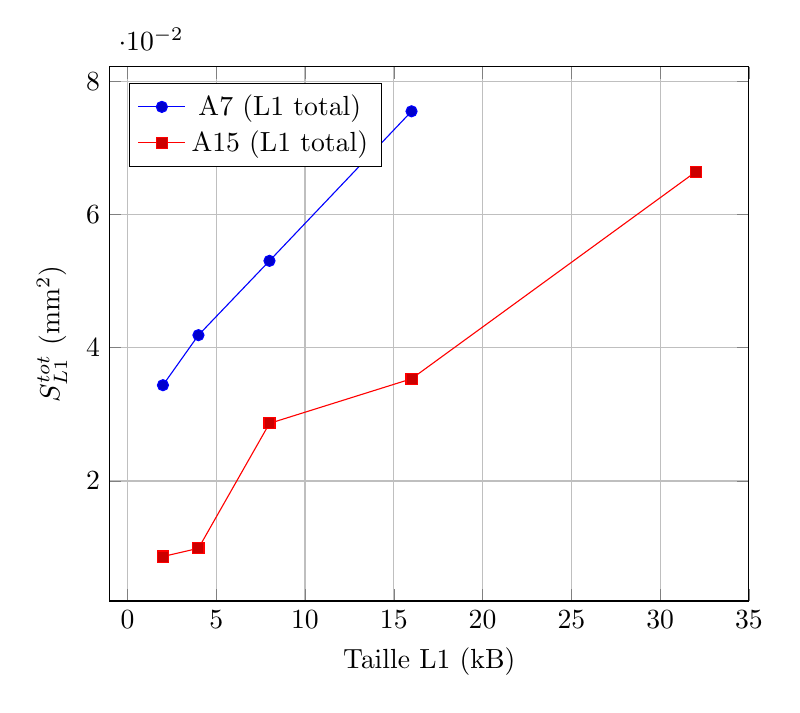
\begin{tikzpicture}
\begin{axis}[
    width=0.8\linewidth,
    xlabel={Taille L1 (kB)},
    ylabel={$S_{L1}^{tot}$ (mm$^2$)},
    legend pos=north west,
    grid=both
]
\addplot coordinates {(2,0.03438) (4,0.04189) (8,0.05304) (16,0.07548)};
\addlegendentry{A7 (L1 total)}
\addplot coordinates {(2,0.00867) (4,0.00990) (8,0.02865) (16,0.03534) (32,0.06639)};
\addlegendentry{A15 (L1 total)}
\end{axis}
\end{tikzpicture}
\caption{Surface totale des L1 (I+D) en fonction de la taille.}
\end{figure}

\begin{figure}[h]
\centering
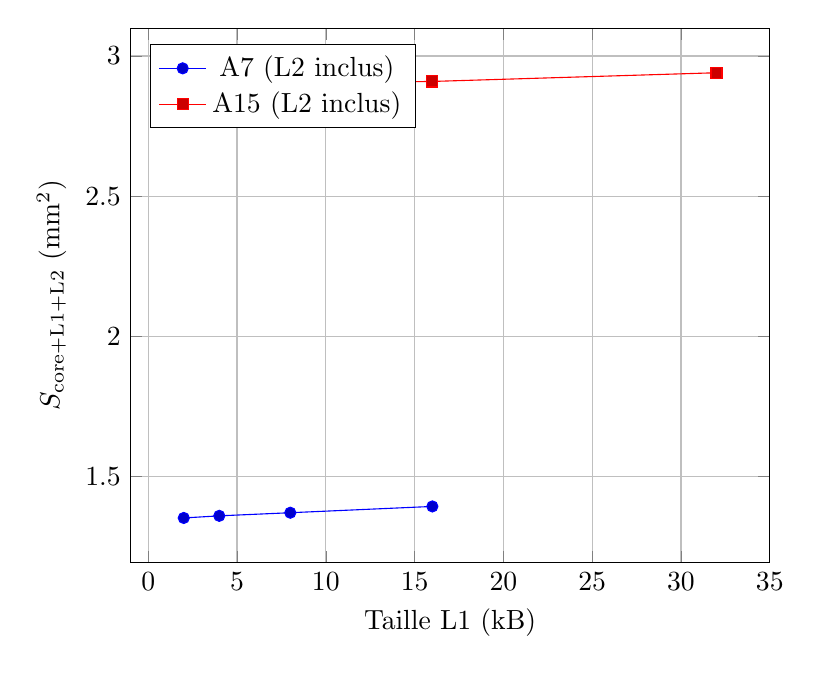
\begin{tikzpicture}
\begin{axis}[
    width=0.8\linewidth,
    xlabel={Taille L1 (kB)},
    ylabel={$S_{\text{core+L1+L2}}$ (mm$^2$)},
    legend pos=north west,
    grid=both
]
\addplot coordinates {(2,1.35130) (4,1.35882) (8,1.36996) (16,1.39241)};
\addlegendentry{A7 (L2 inclus)}
\addplot coordinates {(2,2.88247) (4,2.88370) (8,2.90245) (16,2.90914) (32,2.94019)};
\addlegendentry{A15 (L2 inclus)}
\end{axis}
\end{tikzpicture}
\caption{Surface totale des cœurs (L1 variable + L2=512\,kB).}
\end{figure}


\paragraph{Efficacité surfacique.}
On utilise les IPC issus des fichiers CSV (par processus et par taille de L1) et la surface
totale du cœur avec L2 fixe (512\,kB) :
\[
\eta = \frac{IPC}{S_{\text{total}}}\quad\text{avec}\quad
S_{\text{total}} = S_{\text{core hors L1}} + 2S_{L1} + S_{L2}.
\]
Ici $S_{L2}(A7)=0{,}94241$~mm$^2$ et $S_{L2}(A15)=0{,}94019$~mm$^2$.
Les valeurs suivantes sont donc en $IPC/\text{mm}^2$.

\begin{table}[h]
\centering
\footnotesize
\begin{tabular}{c|cccc}
\hline
\textbf{L1 (kB)} & \textbf{Dijkstra small} & \textbf{Dijkstra large} & \textbf{Blowfish small} & \textbf{Blowfish large} \\
\hline
\multicolumn{5}{c}{\textbf{Cortex-A7}}\\
1  & --      & --      & --      & -- \\
2  & 0,1787  & 0,1778  & 0,1859  & 0,1902 \\
4  & 0,1860  & 0,1846  & 0,1943  & 0,1983 \\
8  & 0,2006  & 0,1989  & 0,2127  & 0,2162 \\
16 & 0,2025  & 0,2009  & 0,2102  & 0,2138 \\
\hline
\end{tabular}
\caption{Efficacité surfacique du Cortex-A7 (L2=512\,kB).}
\end{table}

\begin{table}[h]
\centering
\footnotesize
\begin{tabular}{c|cccc}
\hline
\textbf{L1 (kB)} & \textbf{Dijkstra small} & \textbf{Dijkstra large} & \textbf{Blowfish small} & \textbf{Blowfish large} \\
\hline
\multicolumn{5}{c}{\textbf{Cortex-A15}}\\
2  & 0,2249  & 0,2269  & 0,3487  & 0,3667 \\
4  & 0,2516  & 0,2500  & 0,3710  & 0,3915 \\
8  & 0,3253  & 0,3129  & 0,4444  & 0,4669 \\
16 & 0,3516  & 0,3386  & 0,4523  & 0,4763 \\
32 & 0,3908  & 0,3907  & 0,4820  & 0,5094 \\
\hline
\end{tabular}
\caption{Efficacité surfacique du Cortex-A15 (L2=512\,kB).}
\end{table}

\textit{Note :} CACTI ne fournit pas d’organisation valide pour A7 à 1\,kB, d’où ``--''.

\section{Efficacité énergetique.}

\subsection{Puissance en mW consomme par chaque processeur à la fréquence maximale}
Les consommations \'energ\'etiques du Cortex-A7 et du Cortex-A15 sont de 0{,}10~mW/MHz et 0{,}20~mW/MHz, respectivement. De plus, en technologie 28~nm, les fr\'equences maximales du Cortex-A7 et du Cortex-A15 sont de 1{,}0~GHz et 2{,}5~GHz, respectivement. La puissance \`a fr\'equence maximale pour chaque microprocesseur peut \^etre estim\'ee comme suit.

Le calcul de la puissance \`a fr\'equence maximale ($P_{\max}$) est donn\'e par l’\'equation \eqref{eq:pmax} :
\begin{equation}
P_{\max}=\left(\frac{\text{mW}}{\text{MHz}}\right)\times \left(\text{MHz}\right)
\label{eq:pmax}
\end{equation}

\noindent
\textbf{1.~Cortex-A7 :} en appliquant l’\'equation \eqref{eq:pmax}, on obtient :
\begin{equation}
P_{A7}=0{,}10~\frac{\text{mW}}{\text{MHz}}\times 1000~\text{MHz}=100~\text{mW}
\label{eq:pa7}
\end{equation}

\noindent
\textbf{2.~Cortex-A15 :} de la m\^eme mani\`ere, on obtient :
\begin{equation}
P_{A15}=0{,}20~\frac{\text{mW}}{\text{MHz}}\times 2500~\text{MHz}=500~\text{mW}
\label{eq:pa15}
\end{equation}

\`A partir de cette puissance \`a fr\'equence maximale, il est possible d’estimer l’efficacit\'e \'energ\'etique \`a l’aide de la formule donn\'ee \`a l’\'equation \eqref{eq:eff_energetique} :
\begin{equation}
E = \frac{\mathrm{IPC}}{P_{\max}}
\label{eq:eff_energetique}
\end{equation}

\subsection{Configuration de L1 l’efficacité énergétique de chaque processeur (à fréquence maximale).}
Cette expression est appliqu\'ee \`a toutes les applications, pour chacune des configurations dans lesquelles elles ont \'et\'e simul\'ees.


\begin{table}[H]
\centering
\footnotesize
\resizebox{\linewidth}{!}{%
\begin{tabular}{c|c|c|c|c}
\hline
\textbf{L1 (kB)} & \textbf{Dijkstra small} & \textbf{Dijkstra large} & \textbf{Blowfish small} & \textbf{Blowfish large} \\
\hline
1  & 0,00232 & 0,00232 & 0,00245 & 0,00251 \\
2  & 0,00244 & 0,00240 & 0,00251 & 0,00257 \\
4  & 0,00254 & 0,00250 & 0,00264 & 0,00270 \\
8  & 0,00275 & 0,00272 & 0,00291 & 0,00296 \\
16  & 0,00283 & 0,00279 & 0,00293 & 0,00298 \\
\hline
\end{tabular}
}
\caption{Efficacite energetique (IPC/mW) pour Cortex-A7 ($P_{\max}$ = \mbox{100\,mW}).}
\label{tab:eff-energetique-a7}
\end{table}

\begin{table}[H]
\centering
\footnotesize
\resizebox{\linewidth}{!}{%
\begin{tabular}{c|c|c|c|c}
\hline
\textbf{L1 (kB)} & \textbf{Dijkstra small} & \textbf{Dijkstra large} & \textbf{Blowfish small} & \textbf{Blowfish large} \\
\hline
2  & 0,00130 & 0,00131 & 0,00201 & 0,00211 \\
4  & 0,00145 & 0,00143 & 0,00214 & 0,00226 \\
8  & 0,00190 & 0,00181 & 0,00258 & 0,00271 \\
16  & 0,00207 & 0,00196 & 0,00263 & 0,00277 \\
32  & 0,00232 & 0,00229 & 0,00283 & 0,00300 \\
\hline
\end{tabular}
}
\caption{Efficacite energetique (IPC/mW) pour Cortex-A15 ($P_{\max}$ = \mbox{500\,mW}).}
\label{tab:eff-energetique-a15}
\end{table}


On a conclu qu’en d\'efinissant l’efficacit\'e du projet \`a partir de l’IPC et de la puissance consomm\'ee \`a la fr\'equence maximale, on obtient les r\'esultats attendus. En effet, plus la taille du cache augmente, plus l’IPC s’am\'eliore et, avec un d\'enominateur constant (ou fix\'e), l’efficacit\'e \'energ\'etique augmente pour les deux microprocesseurs.

Par ailleurs, il est important de souligner que, pour la plupart des tailles de cache comparables entre les deux architectures propos\'ees, l’efficacit\'e \'energ\'etique du microprocesseur A15 est inf\'erieure \`a celle du microprocesseur A7.

\subsection{Analyse critique et initiative technique}
Si l’on s’en tient strictement \`a la m\'etrique impos\'ee par l’\'enonc\'e (\(\mathrm{IPC}/\mathrm{mW}\)), le Cortex-A7 appara\^it comme le plus efficace, ce qui est coh\'erent avec son positionnement \emph{low power}.

Pour cette comparaison, nous fixons explicitement les deux points de r\'ef\'erence suivants issus des simulations Gem5 sur \emph{Dijkstra large} :
\begin{itemize}
\item Cortex-A7 : \(\mathrm{IPC}=0.275495\).
\item Cortex-A15 avec \(L1=32~\mathrm{kB}\) : \(\mathrm{IPC}=1.158855\).
\end{itemize}

Cependant, en tant que concepteurs syst\`eme, ce r\'esultat doit \^etre nuanc\'e. La m\'etrique \(\mathrm{IPC}/\mathrm{mW}\) normalise par la puissance mais n’int\`egre pas explicitement l’effet de la fr\'equence d’horloge. Or, le Cortex-A15 fonctionne \`a \(2.5\times\) la fr\'equence du Cortex-A7.

Pour obtenir une vision plus r\'ealiste du compromis performance/\'energie, nous introduisons donc le ratio \emph{performance r\'eelle par watt} en \(\mathrm{GIPS}/\mathrm{W}\).

\textbf{1. Performance r\'eelle (GIPS)}
\[
\mathrm{GIPS} = \mathrm{IPC}\times f\;(\mathrm{GHz})
\]
\[
\text{A7: }0.275495 \times 1.0 = 0.275495\;\mathrm{GIPS}
\]
\[
\text{A15: }1.158855 \times 2.5 = 2.8971375\;\mathrm{GIPS}
\]
Le Cortex-A15 est donc environ \(10.52\times\) plus rapide en d\'ebit absolu.

\textbf{2. Efficacit\'e r\'eelle \((\mathrm{GIPS}/\mathrm{W})\)}
\[
\eta_{\text{r\'eelle}} = \frac{\mathrm{GIPS}}{P\;(\mathrm{W})}
\]
\[
\text{A7: }\frac{0.275495}{0.1} = 2.75495\;\mathrm{GIPS/W}
\]
\[
\text{A15: }\frac{2.8971375}{0.5} = 5.794275\;\mathrm{GIPS/W}
\]

Cette initiative montre que, malgr\'e un avantage apparent de l’A7 en \(\mathrm{IPC}/\mathrm{mW}\), l’A15 d\'elivre une meilleure performance utile par watt lorsque la fr\'equence est prise en compte. En pratique, le choix final d\'epend donc de l’objectif syst\`eme : minimiser la puissance instantan\'ee (A7) ou maximiser le d\'ebit \'energ\'etique global (A15).

\section{Architecture système big.LITTLE}
En s’inscrivant dans l’approche ARM \emph{big.LITTLE}, on propose de s\'electionner, pour chacune des applications, une configuration de cache L1 pouvant \^etre int\'egr\'ee dans chaque cluster, en traitant les applications s\'epar\'ement. Cette s\'election s’appuie sur les r\'esultats d’efficacit\'e \'energ\'etique obtenus pour les diff\'erentes configurations, pour chacune des applications.
\subsection{Dijkstra big.LITTLE}
Ainsi, dans le cas de Dijkstra, pour le cluster \emph{little}, c’est-\`a-dire le Cortex-A7, on propose une configuration avec une I-cache et une D-cache de 16~kB. En effet, c’est \`a 16~kB de D-L1 que l’on obtient la meilleure efficacit\'e \'energ\'etique ainsi que la meilleure efficacit\'e surfacique, aussi bien pour Dijkstra \emph{Small} que pour Dijkstra \emph{Large}.

Il convient de souligner que ces r\'esultats sont coh\'erents avec ceux obtenus lors de l’analyse de performance du Cortex-A7 face aux variations de la taille du cache pour Dijkstra. N\'eanmoins, une nuance m\'erite d’\^etre prise en compte. Lors de l’analyse de Dijkstra \emph{Small} et \emph{Large}, on a observ\'e que le gain d’IPC entre un L1 de 8~kB et un L1 de 16~kB n’est pas suffisamment significatif pour constituer un crit\`ere d\'eterminant en termes de performance.

Cela s’explique par le fait qu’un point d’inflexion appara\^\i t autour de 8~kB et qu’\`a partir de 16~kB la progression de l’IPC commence \`a saturer. Par cons\'equent, puisque les diff\'erences d’efficacit\'e surfacique et d’efficacit\'e \'energ\'etique entre 8~kB et 16~kB ne sont pas consid\'erables (les valeurs \'etant tr\`es proches), la s\'election entre ces deux tailles peut \^etre laiss\'ee \`a d’autres crit\`eres de conception, notamment des consid\'erations de co\^ut pour le fabricant ou des besoins sp\'ecifiques. En effet, les performances en simulation sont tr\`es similaires et, de plus, les indicateurs d’efficacit\'e surfacique et d’efficacit\'e \'energ\'etique restent tr\`es proches l’un de l’autre.

Pour le cluster \emph{big}, c’est-\`a-dire le processeur Cortex-A15, dans le cas particulier de l’application Dijkstra, on propose une configuration de 32~kB pour le cache d’instructions et le cache de donn\'ees, principalement pour trois raisons.

Premi\`erement, c’est avec cette configuration que l’on atteint la meilleure efficacit\'e surfacique parmi toutes les configurations \'evalu\'ees pour cette application sur Cortex-A15. Deuxi\`emement, il s’agit \'egalement de la configuration offrant la meilleure efficacit\'e \'energ\'etique pour ce microprocesseur et cette application, ce qui est coh\'erent avec les r\'esultats de performance obtenus pour Dijkstra \emph{Large} et \emph{Small}. Troisi\`emement, la hausse de l’IPC atteint 74{,}99\% lorsque la taille du cache est de 32~kB, et l’on n’observe pas encore une saturation compl\`ete de la diminution des pertes, en particulier pour la D-cache. Or, pour cette configuration et sur ce microprocesseur, c’est pr\'ecis\'ement la r\'eduction des pertes en D-cache qui constitue la source principale du gain d’IPC.

Par cons\'equent, cette configuration repr\'esente l’option recommand\'ee : elle maximise non seulement le gain d’IPC, mais aussi la diminution des pertes en cache de donn\'ees et en cache d’instructions, tout en maximisant l’efficacit\'e \'energ\'etique et l’efficacit\'e surfacique.
\subsection{Blowfish big.LITTLE}
Dans le cas sp\'ecifique des applications Blowfish, \emph{Small} comme \emph{Large}, sur le cluster \emph{little} (Cortex-A7), on obtient une situation particuli\`ere. En effet, l’efficacit\'e surfacique maximale est atteinte avec une configuration de cache de 8~kB, tandis que l’efficacit\'e \'energ\'etique maximale, dans le cadre d’une puissance suppos\'ee constante \`a la fr\'equence maximale de fonctionnement du microprocesseur, est obtenue avec une configuration de 16~kB.

Par cons\'equent, un troisi\`eme crit\`ere est retenu pour s\'electionner la configuration recommand\'ee : le comportement en performance observ\'e lors de l’analyse du microprocesseur face \`a cette application pour diff\'erentes tailles de cache. On avait montr\'e qu’\`a partir de 8~kB, un point d’inflexion est atteint et qu’augmenter la taille du cache ne produit plus de gains significatifs en termes d’IPC. De plus, on observe une saturation \`a la fois de la diminution des pertes en I-cache et de la diminution des pertes en D-cache, ce qui rend peu pertinent, du point de vue des performances applicatives, d’int\'egrer une configuration \`a cache plus grand.

C’est pourquoi, pour Blowfish sur Cortex-A7, on recommande une configuration de 8~kB pour la I-cache et de 8~kB pour la D-cache.

Pour Blowfish sur le cluster \emph{big} (Cortex-A15), la configuration recommand\'ee est de 32~kB pour la I-cache et 32~kB pour la D-cache, pour trois raisons principales.

Premi\`erement, avec cette configuration, on obtient la meilleure efficacit\'e surfacique, dans le cadre d’une puissance suppos\'ee constante \`a la fr\'equence maximale. Deuxi\`emement, cette m\^eme configuration pr\'esente aussi la meilleure efficacit\'e \'energ\'etique pour cette application, aussi bien en version \emph{Small} qu’en version \emph{Large}. Enfin, ces r\'esultats sont coh\'erents avec l’analyse de performance, qui montre que le gain d’IPC continue jusqu’\`a la configuration L1 de 32~kB, atteignant une am\'elioration de 41{,}68\%. Bien que cette taille mette en \'evidence une certaine saturation de la diminution des pertes en D-cache et en I-cache, elle ne montre pas encore une saturation (ou un \'etat de stagnation) du gain d’IPC.

Par cons\'equent, il reste pertinent, en termes de performance, de mettre en \oe{}uvre un cache de 32~kB plut\^ot qu’un cache de 16~kB. Ce dernier n’apporte qu’un gain d’IPC de 31{,}017\%, soit environ 10 points de pourcentage de moins. L’ensemble de ces \'el\'ements renforce ainsi la d\'ecision retenue pr\'ec\'edemment.










Dans le cas des configurations du cluster \emph{big}, elles sont \'equivalentes pour Blowfish comme pour Dijkstra. Cela s’explique par le fait que, dans les deux applications, le goulot d’\'etranglement se situait principalement au niveau des instructions de calcul entier. Ainsi, l’impl\'ementation du Cortex-A15 et sa capacit\'e \`a traiter davantage d’instructions en parall\`ele permettent des am\'eliorations d’IPC consid\'erables, ce qui rend la dynamique d’am\'elioration des acc\`es aux donn\'ees en m\'emoire plus visible.

M\^eme si la nature des structures de donn\'ees manipul\'ees et les modes d’acc\`es \`a la m\'emoire diff\`erent entre les deux algorithmes, les r\'esultats ne sont pas n\'ecessairement identiques, mais ils suivent un comportement incr\'emental du m\^eme type jusqu’\`a atteindre la configuration optimale retenue, \`a savoir 32~kB. N\'eanmoins, ces diff\'erences de structures et de sch\'emas d’acc\`es montrent qu’apr\`es l’adoption de ce microprocesseur, les gains d’IPC obtenus en augmentant la taille du cache sont plus repr\'esentatifs pour Dijkstra que pour Blowfish. Malgr\'e cela, les deux applications conservent la m\^eme taille optimale de cache, c’est-\`a-dire la configuration \`a 32~kB.

De son c\^ot\'e, pour le cluster \emph{little}, la configuration de cache recommand\'ee n’est pas la m\^eme, en se basant principalement sur l’efficacit\'e surfacique. En effet, pour Blowfish \emph{Small} et \emph{Large} sur Cortex-A7, l’efficacit\'e surfacique est plus \'elev\'ee lorsque la configuration du cache est de 8~kB, ce qui diff\`ere des r\'esultats obtenus pour Dijkstra sur ce m\^eme microprocesseur. Par cons\'equent, la recommandation initiale est diff\'erente.

N\'eanmoins, les performances obtenues avec les configurations \`a 8~kB restent comparables, et l’on pourrait m\^eme envisager l’utilisation d’une configuration de 8~kB pour Dijkstra. En effet, en termes de performance, une fois ce point d’inflexion d\'epass\'e, les gains d’IPC tendent \`a se saturer, ce qui rend les diff\'erences entre 8~kB et des tailles sup\'erieures moins marqu\'ees.

Le point d’inflexion observ\'e pour Dijkstra autour de 8~kB sur Cortex-A7 s’interpr\`ete comme une forme de saturation des gains d’IPC. Par cons\'equent, l’\'ecart entre une configuration de 8~kB et une configuration de 16~kB n’est pas repr\'esentatif en termes de performance. De plus, l’efficacit\'e \'energ\'etique demeure \'egalement comparable entre ces deux tailles.

Ainsi, m\^eme si la configuration recommand\'ee n’est pas strictement \'equivalente, il serait envisageable d’impl\'ementer Dijkstra avec une configuration de 8~kB sur Cortex-A7, puisqu’elle n’entra\^\i nerait ni un co\^ut important en performance, ni un co\^ut notable en efficacit\'e \'energ\'etique, par comparaison avec la configuration recommand\'ee.

\subsection{Méthodologie de Spécification Architecturale}
Pour sp\'ecifier une architecture d\'edi\'ee \`a un nouveau domaine (par exemple l’intelligence artificielle ou le traitement vid\'eo), nous proposons la m\'ethodologie rigoureuse suivante, d\'eriv\'ee de l’exp\'erience acquise lors de ce TP :

\begin{enumerate}
  \item \textbf{Caract\'erisation de la charge (\emph{profiling}).} Utiliser des outils comme Gem5 (mode atomique) pour extraire le ``mix d'instructions''.
  
  \textit{Objectif :} identifier si l’application est \emph{compute-bound} (n\'ecessitant des ALU/FPU plus larges) ou \emph{memory-bound} (n\'ecessitant des caches et de la bande passante).

  \item \textbf{Exploration de l’espace de conception (\emph{Design Space Exploration}, DSE).} Automatiser les simulations (via des scripts Python/Bash comme dans ce TP) en faisant varier les param\`etres critiques : taille de cache, largeur de pipeline (\emph{issue width}), pr\'edicteurs de branchement. Mesurer l’IPC pour chaque point.

  \item \textbf{Contraintes physiques (PPA : \emph{Power, Performance, Area}).} Mod\'eliser chaque configuration retenue avec un outil physique comme CACTI~7.0 (pour la surface et la latence) et McPAT (pour la puissance). Rejeter les configurations irr\'ealistes (par exemple, latence $>1$ cycle).

  \item \textbf{Analyse de Pareto et choix final.} Tracer les courbes de compromis (par exemple, performance vs surface). S\'electionner les points du front de Pareto : ceux qui offrent le meilleur gain de performance pour un co\^ut marginal en surface/\`energie acceptable. \`A titre d’exemple dans ce TP, le passage de 16~kB \`a 32~kB sur le Cortex-A15 \'etait sur le front de Pareto (gain tr\`es important), alors que sur le Cortex-A7 il ne l’\'etait pas (gain n\'egligeable).
\end{enumerate}

\begin{thebibliography}{00}
\bibitem{Profiling} M. J. P. (University of York), ``Profiling,'' \emph{Lecture Notes (4th Year HPC), University of York}. [Online]. Available: https://www-users.york.ac.uk/\textasciitilde{}mijp1/teaching/4th\_year\_HPC/lecture\_notes/Profiling.pdf. Accessed: Feb. 9, 2026.
\end{thebibliography}
\end{document}
